\ifdefined\included
\else
\setcounter{chapter}{7} %% Numéro du chapitre précédent ;)
\dominitoc
\faketableofcontents
\fi

\chapter{Moving forward binary relations in the REG}
\minitoc
\label{chap:7}

A number of works trend to semantically represent and describe robots' actions and task using ontology. However, each representation has its own particularity, depending on the system it is used on and the exploitation it aims to enable. While our description of past activities fits our needs and our task planner, having a REG algorithm constraint by this latter is problematic. In this chapter we explore the use of n-ary relation, a common, even not yet standard, way to represent complex knowledge as actions. With the analyse of such a pattern, we present a novel REG approach, supporting the use of past activities, but also any complex knowledge represented through n-ary relations.

The contribution presented in this chapter is a preliminary work aiming to consider the limitations encountered by the contribution of the previous chapter. The presented method has been implemented but not tested with an integration of other components. This section deviates a little from the field of \acrshort{hri} to be more anchored in artificial intelligence. However, the ability to generate entity referencing in a more generic way is paramount for a robot to interact with humans. 

\section{Introduction}

Representing the whole complexity of the knowledge composing our world into a machine-readable language is a central issue in artificial intelligence. Coming from the Semantic Web, we saw that the use of an ontology through RDF-based languages succeeded in establishing itself in the field of artificial intelligence and therefore robotics. Although, what is often viewed as a limitation of ontology is its capability to only represent unary and binary relations. Binary relations such as \textit{``Sean Connery has the British nationality''} are described through the form of triples \textit{(sean\_connery, hasNationality, british)}. Unary relation such as \textit{``Sean Connery is an actor''} can them be transformed into binary relation through the addition of dedicated predicates \textit{(sean\_connery, isA, Actor)}. However, the description of more complex relations involving more than two entities is must more challenging using such representation.

Taking the example of Sean Connery\footnote{In the case you do not know who is Sean Connery feel free to take another actor that you like but you will have to adapt the entire example. Good luck.}, f we want to refer to him\footnote{Obviously we want to refer to him without his name since we consider a person having recognized himself in the previous note.}, we could state that he is the actor playing the role of James Bond. However, other actor played this role. We could also say that he is the actor playing in the film Gold finger but once again others do. We could finally explain that he is the actor playing the role of James Bond and playing in the film Gold Finger. However, limiting us to the use of binary relations modify the exact information. A more accurate description would be that he is the actor playing the role of James Bond in the film Gold Finger. Here we see the necessity of relations involving more than two entities. In our example, we need to link the three entities that are the actor ``Sean Connery'', the role ``James Bond'', and the film ``Gold Finger''. Together, they describe a performance. Without being explicitly linked all three theses information would not represent the performance. Moreover, without these links, we could give an explanation such as the actor playing the role of James Bond and playing in the film Rising Sun. Both information is true but does not make sense together.

To refer to an entity, being an object or an agent, such complex relations could be useful but have to be managed carefully to keep the link between each binary relation composing it. In the light of this consideration, we can observe that the description of past agent tasks used in the previous chapter is based on the same principle. Where we refer to Sean Connery through his role and the film he plays in, we have described the knife through the vegetable it has been to cut and the agent having used it. However, depending on the context of the conversation, is it not always necessary to use all the binary relations of such a complex one. We may need only one. Trying to list the actors having the honorific title of ``Sir'', the referring expression \textit{``The man having played James Bond''} could be sufficient. In the same way, to designate the knife, the sentence \textit{``The knife you cut with''} could also be sufficient in some context.

In this chapter, we will try to generalise the \acrshort{reg} algorithm to deal with non-binary relations and pass over the limitations of the previous chapter. The algorithm has to be more generic should no more have any apriori of concepts and properties of the used ontology.
First, we review the literature concerning the representation of non-binary relation in the ontology. Then, we define what we will call a \acrlong{cr} and how we can represent it. The modified algorithm is then detailed before ending with an efficiency comparison regarding the original version and the extended one.

\section[Related work]{Related work: A richer knowledge representation with n-ary relations}

A fundamental feature of relations is their \textbf{arity}. It is the number of individuals they involved~\cite{giunti_2019_representing}. In this sense, unary relations involved only one entity while binary relation involves two entities\footnote{The entities involved in a relation do not have to be distinct. If the same entity is used twice in the same relation the relation is still a binary relation}. What interest us here is n-ary relations with arity $n > 2$.

Well before being treated for ontology used that it is in RDF or OWL, several approaches have been proposed in the field of Artificial Intelligence through the use of semantic network\footnote{Here we close the loop with the hypothesis by Collins and Quillian of the structure of the semantic memory to be like a semantic network.}~\cite{brachman_1979_epistemological, sowa_2014_principles}. Deliyanni and Kowalski~\cite{deliyanni_1979_logic} were the first to explicitly treat the representation of n-ary relations with arity $n > 2$. They propose a semantic network composed of an element representing the relation itself. In this way, they have represented the assertion ``\textit{John gives the book to Mary}'' with five node and four arrows as illustrated in figure~\ref{fig:chap7_sem_net}. The central node \textit{el} allow linking the four elements of the assertion using only binary relations. The approach is tody know as \textbf{relation reification} and has been used in many applications~\cite{gangemi_2008_norms, welty_2006_reusable}.

\begin{figure}[ht!]
\centering
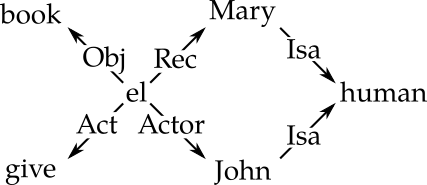
\includegraphics[scale=0.4]{figures/chapter7/semantic_net.png}
\caption{\label{fig:chap7_sem_net} The semantic network used to represent the assertion ``\textit{John gives the book to Mary}''. The element \textit{el} is used to represent the global event.}
\end{figure}

The general idea used in all the proposed approaches since Deliyanni is thus the creation of a \textbf{relation-class} that is instantiated to represent the n-ary relation. Then $n$ binary relations are created to link the $n$ entity to the relation-class instance. For a more global view of the different proposed patterns, you can refer to the survey~\cite{gangemi_2013_multi}.

For the use in ontology, no standard pattern has been approved by the W3C for the moment. However, a Working Group Note has been proposed for the standardisation of such relations in RDF and OWL~\cite{w3c_2006_defining}. In the note, two patterns are introduced with two variants for the first one.

\begin{figure}[ht!]
\centering
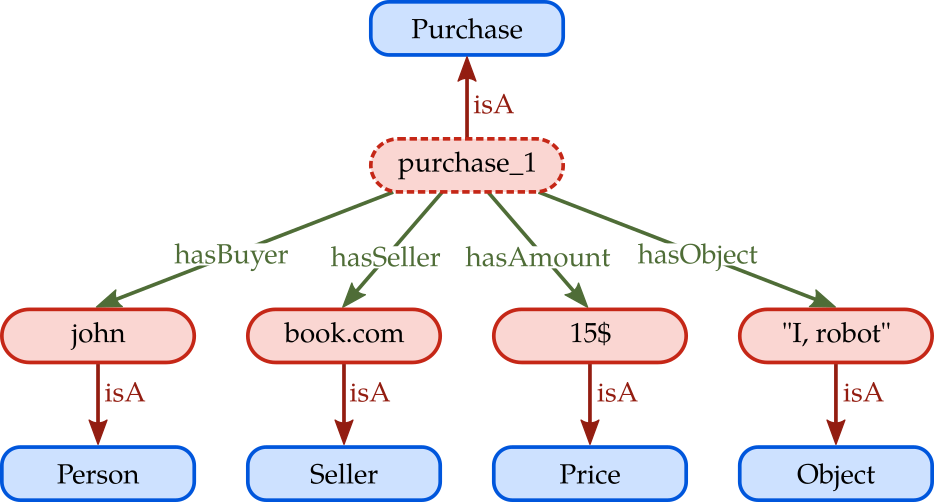
\includegraphics[scale=0.4]{figures/chapter7/w3c_p2.png}
\caption{\label{fig:chap7_w3c_p2} Ontological pattern 1 without subject proposed by the W3C Working Group. The describe assertion is ``John buys a ''I, robot`` from books.com for \$15''.}
\end{figure}

The first pattern is based on the introduction of a new class for relation and works in the exact same way of the relation reification as illustrated in Figure~\ref{fig:chap7_w3c_p2}. The class \textit{Purchase} is a relation-class and its instance \textit{purchase\_1} is link the entities of the relation. Such pattern is said to be \textbf{without subject} as all the relation are oriented from the relation-class instance to the other entities.

\begin{figure}[ht!]
\centering
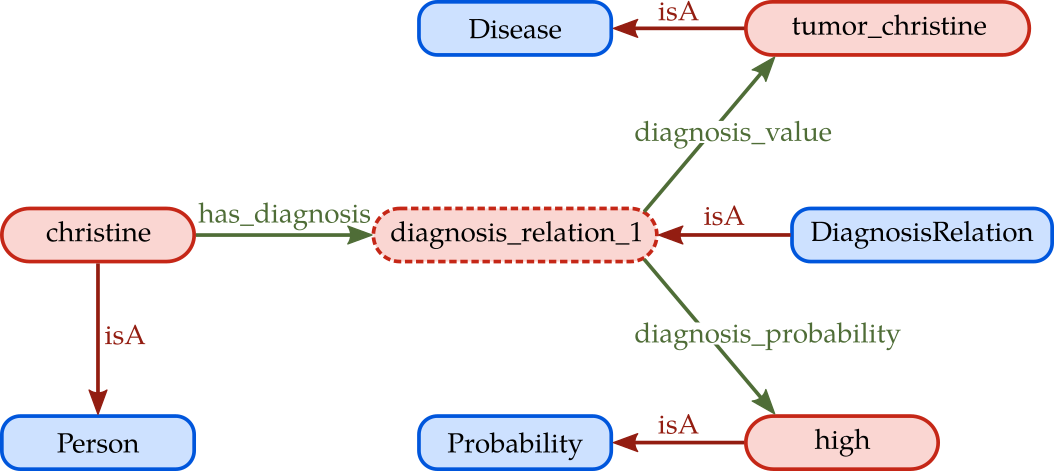
\includegraphics[scale=0.4]{figures/chapter7/w3c_p1.png}
\caption{\label{fig:chap7_w3c_p1} Ontological pattern 1 with subject proposed by the W3C Working Group. The describe assertion is ``Christine has tumor with high probability''.}
\end{figure}


A variation of the first pattern is illustrated in Figure~\ref{fig:chap7_w3c_p1}. This variation is said to be \textbf{with subject}. The assertion described here is ``Christine has a tumor with high probability''. Here the subject of the relation is Christine. It is represented in the pattern by a relation oriented from Christine to the instance of the relation-class while the others are in the usual orientation. Such variation can be reproduced with the previous one by defining inverse relations. Defining the relation \textit{isBuyer} and \textit{isObject}, either John or the book can be the subject of the relation represented by \textit{purchase\_1}.

\begin{figure}[ht!]
\centering
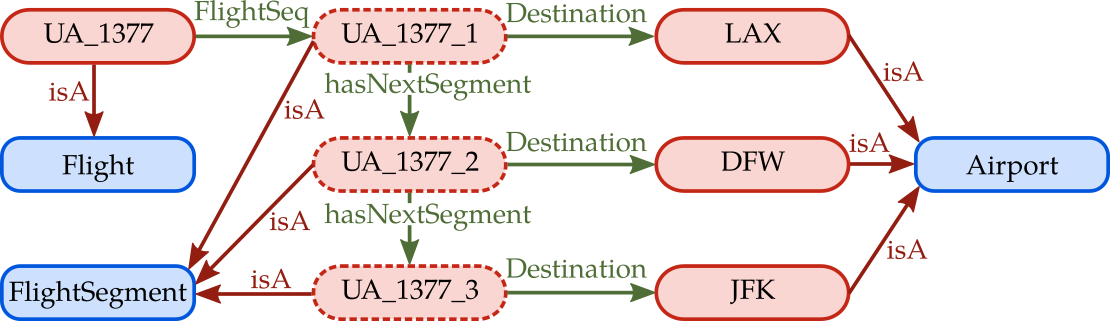
\includegraphics[scale=0.4]{figures/chapter7/w3c_p3.png}
\caption{\label{fig:chap7_w3c_p3} Ontological pattern 2 with subject proposed by the W3C Working Group. The describe assertion is ``United Airlines flight 1377 visits the following airports: LAX, DFW, and JFK''.}
\end{figure}


The second pattern aims at representing lists. With the previous pattern, it is assumed that the properties involved in the binary relation are only used once to identify uniquely each element of the relation. Wanting to represent the assertion ``United Airlines flight 3177 visits the following airports: LAX, DFW, and JFK'' the first pattern would be not adapted. With this other pattern, we create several instances of the relation-class each linked to the next and to an entity of the n-ary relation as illustrated in Figure~\ref{fig:chap7_w3c_p3}. Because one of the binary relations go from an entity of the relation to an instance of the relation-class, it is said to be with subject. This second pattern is dedicated to the description of lists.

\section{Through the use of coumpound relations}

In the rest of the chapter, we consider the n-ary relations with arity $n > 2$ under the name \textbf{\acrfull{cr}} because of the composition of binary relations to represent them on the principle of reification. The term relation will be used to speak about binary relations. We first define what is a \acrshort{cr} in link with the ontology definition and on the base of the first pattern without subject, proposed by the Working Group Note. Then, we present an algorithm to pre-process them with the objective to facilitate their use in the \acrshort{reg} algorithm.

\subsection{Defining a compound relation}

To define the structure of a \acrlong{cr} we take the example of the purchase made by John on the website book.com to buy the book ``I, Robot'' at 15\$. This statement is graphically represented in Fig.~\ref{fig:chap7_cr}a and the underlying pattern in Fig.~\ref{fig:chap7_cr}b. To represent the compound relation, we start by creating a virtual entity (the instance of the relation-class) that will be the common link for all the relations involved in the compound relation. We call this instance entity the \textbf{\acrfull{ce}}. It is the dotted entity on Figure~\ref{fig:chap7_cr}, respectively $purchase\_1$ and $\indiv_c$. We consider as being part of the \acrshort{cr} all the relations for which the \acrshort{ce} is the subject: $(purchase\_1, has\_buyer, john)$. 

\begin{theorem} [Compound Relation]
\label{the:compound_relation}
For any $\indiv_c$ being a Coumpound Entity, a Coumpound Relation is defined by $R_c = \{ \relation_i\ |\  \relation_i = (\indiv_c, \property_i, \indiv_i), \forall \indiv_i \in \indivset\}$ meaning the set of relation composing it.
\end{theorem}

\begin{figure}[ht!]
\centering
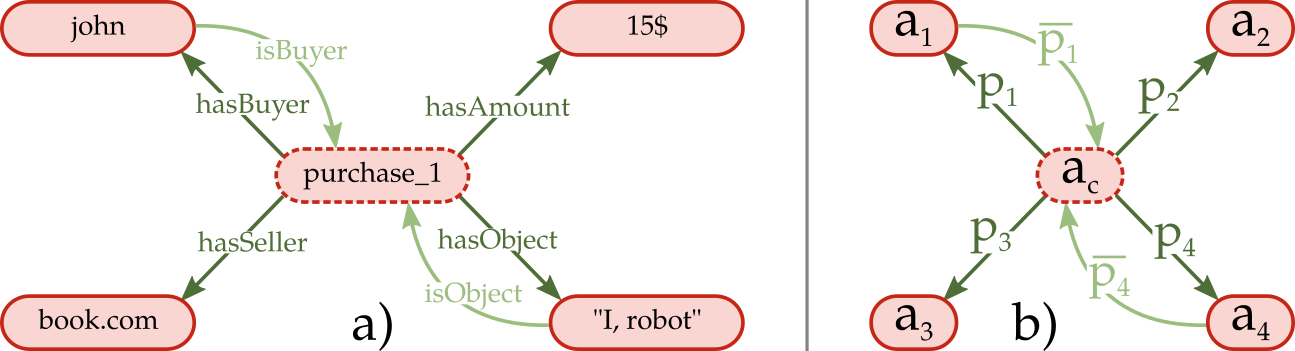
\includegraphics[width=\textwidth]{figures/chapter7/CR.png}
\caption{\label{fig:chap7_cr} The graphical representation of compound relations. The dotted entity at the center of each representation is the so-called compound entity. The outgoing edges are the properties involved in the compound relation. The entering and faded edges are the corresponding inverse properties if any. The compound relation a) describe the purchase made by \underline{John} on the website \underline{book.com} of the book \underline{``I, Robot''} at \underline{15\$}. The compound relation b) is the underlying pattern of the previous example.}
\end{figure}

Regarding the previous definition, because any entity of an ontology could be considered as a \acrshort{ce}, many set of relations without a real link could be considered as a \acrshort{cr}. To solve it, we could define an upper class common the all the \acrshort{ce}, meaning the upper \textit{RelationClass}. However, what better defines a \acrshort{cr} is that to speak about one of its involved entities through it, we have to use other relation of the \acrshort{cr}. In other words, to speak about Sean Connery using the role of James Bond, we have to speak about ``Gold Finger'' rather than ``Murder on the Orient Express'' because even if he played in both films, he played the said role only in the first-mentioned film. At the difference, the relation representing his nationality can be used independently to other relations. To represent this verbal link, Giunti et .al \cite{giunti_2019_representing} introduce an \textit{parametric pattern} on top of n-ary relations (Compound Relations). Their parametric pattern for the purchase example is the following : \textit{``() bought a () from () for ()''}. While as humans we easily identify the place of each entity in the pattern, it is a more complex task for machines. This choice of pattern is explained by their complex representation where they assign a position to each involved relation. Regardless of the representation complexity, this kind of pattern raises two issues. First, the pattern describes the entire \acrshort{cr} and not aims to describe one of the involved entity through the \acrshort{cr} (e.g. ``\textit{() who bought a () from () for ()}''). Second, the pattern necessary involved all the relations composing the \acrshort{cr}, while in the context of the \acrshort{reg}, we could only need a part of them (e.g. \textit{``() who bought a ()}'' if John is the only one who bought this book in the present context).

\subsection{A light way of representing the verbal link}

To represent the verbal link, we also choose to use parametric patterns, patterns for short. The patterns are defined as labels in the ontology. A \acrshort{cr} can have multiple labels (i.e. patterns) depending on the subject of the pattern and the involved relations in the verbal link. The labels are not directly applied to the \acrshort{ce} but to a class, it's inheriting. This means that all the entities inheriting from a class having its labels respecting the pattern are \acrshort{ce}. In a way, we define here a relation-class but one the only base of labels.

\begin{theorem} [Compound Entity]
\label{the:compound_entity}
Given $\omega$ being a pattern, an entity $\indiv_c$ is a \acrlong{ce} iif $\exists \class \in \classset | (\indiv_c, \class) \in \inheritset \land \omega \in \tlabel{(\class)}$
\end{theorem}

An advantage of this solution is that we do not define any new specific concepts or properties in the ontology meaning that any pre-existing ontology can be updated to be used in the \acrshort{reg} process with \acrshort{cr} only by adding labels. Our patterns have the following form : $\{?\property_4\}\ bought\ on\ \{\property_3\}\ by\ \{\property_1\}$. This pattern directly integrates the properties which can be used to form the relations composing the \acrshort{cr}.

Given a compound entity $a_c$ with the previous label, to generate a referring expression using it, the place-holder $\{\property_3\}$ should be replaced by a referring expression of an entity $\indiv_i$ where $\indiv_i$ is the object of a triple $(\indiv_c,\ \property3,\ \indiv_i)$. Because we assume that a property can only appear once in a \acrshort{cr}, we know that there is only one such object $\indiv_i$. In our example, we have $\indiv_i = \indiv_3$ for the $a_c$ \acrshort{ce}.
In this way, without predefined order, an algorithm can easily replace the place-holders by the \acrshort{re} of the entities $\indiv_i$ of the relations $(\indiv_c, \property_i, \indiv_i)$ of the \acrshort{cr}.

Since we are in the context of \acrshort{reg}, the \acrshort{cr} will be used as a reference to one of the entities involved in the \acrshort{cr}. This specific entity is called the \textbf{subject entity} of the \acrshort{cr}. 
For a subject entity to exist, an inverse property $\overline{\rm \property_i}$ must exists in the way that $(\property_i, \overline{\property_i}) \in \invset$ and $\relation_i = (\indiv_i, \overline{\property_i}, \indiv_c) \in \relationset$. If $\indiv_i$ is the subject entity, $\property_i$ is thus the \textbf{subject property} of the \acrshort{cr} and is prefixed with a question mark in the pattern. In the example of Figure~\ref{fig:chap7_cr}, only $\indiv_1$ and $\indiv_4$ (resp. John and the book) can be subject of the \acrshort{cr}. In other words, only these entities can be referred through the use of this \acrshort{cr}. Among all the labels available to speak about the \acrshort{cr}, the usable ones to speak about an entity are the ones for which the corresponding property is the subject property (i.e. prefixed by a question mark in the patterns). This choice to not consider the first in the pattern has been made to be adapted to any language. Among the possible labels of List.\ref{lst:chap7_john_labels}, the patterns L1 to L5 could thus be used as a reference for $\indiv_4$ (the book in our example) while the patterns L6 and L7 could be used as a reference for $\indiv_1$ (John in our example).

\begin{lstlisting}[frame=single, caption={ A part of the label set of the purchase compound relation.}, label={lst:chap7_john_labels}, captionpos=b, style=Labels, mathescape=true]
L1 - {?$p_4$} bought on {$p_3$} at {$p_2$}
L2 - {?$p_4$} bought by {$p_1$}
L3 - {?$p_4$} bought on {$p_3$} by {$p_1$}
L4 - {$?p_4$} bought at {$p_2$} on {$p_3$} by {$p_1$}
L5 - {$?p_4$} bought at {$p_2$} by {$p_1$}
L6 - {$?p_1$} who bought {$p_4$}
L7 - {$?p_1$} who bought {$p_4$} on {$p_3$}
\end{lstlisting}

\subsection{A strategy to explore compund relations}

In a graph exploration, an important parameter to avoid a combinatorial explosion is the branching factor. For the \acrshort{reg} problem, an advantage of \acrshort{cr} is that once we introduce a \acrshort{cr} in the search algorithm we can directly know the relations involved in it. In this sub-section, our goal is thus to analyze the labels in the way to define the order in which the relations of the \acrshort{cr} will be explored by the upper algorithm. By doing so, we will reduce its branching factor and thus avoid any combinatorial explosion of the \acrshort{reg} algorithm.

\subsubsection{A naive strategy to explore compound relations}

Suppose we want to refer to the entity $\indiv_4$ using the compound relation embodied by the compound entity $\indiv_c$ of Figure~\ref{fig:chap7_cr}. This is made possible by the triplet $(\indiv_c,\property_4,\indiv_4)$ in the knowledge-base and its inverse $(\indiv_4, \overline{\property_4}, \indiv_c)$. The listing~\ref{lst:chap7_john_labels} presents some alternative ways in which we can verbalise entities through the \acrshort{cr}. In order to refer $\indiv_4$, we can only use the ones where $\property_4$ is the subject property. Thus the labels L1 to L5 are the only ones that we can use. The parts of the compound relation used by labels L1 and L3 are illustrated in Figure~\ref{fig:chap7_cr_part}.

\begin{figure}[ht!]
\centering
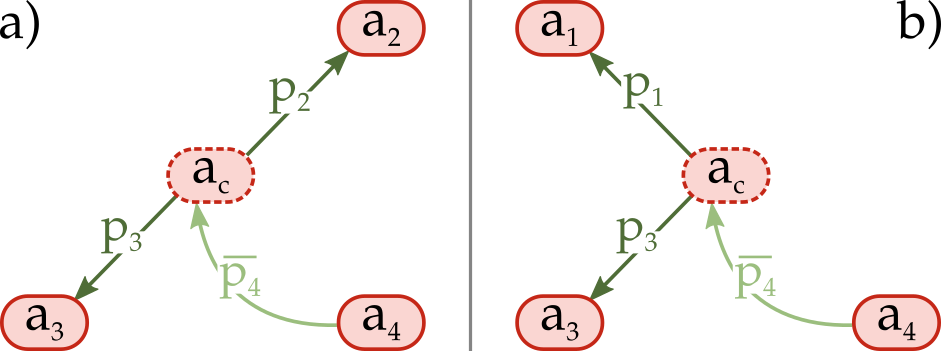
\includegraphics[scale=0.4]{figures/chapter7/CR_part.png}
\caption{\label{fig:chap7_cr_part} The parts of the compound relation used in the label patterns L1 (a) and L3 (b).}
\end{figure}

What interest us in these labels are the properties because it is they that will form the relations to explore. From the patterns in listing~\ref{lst:chap7_john_labels}, we know that we can use label L1 to verbalize the triple set \textit{\{($\indiv_c$,$\property_4$,$\indiv_4$) ($\indiv_c$,$\property_3$,$\indiv_3$) ($\indiv_c$,$\property_2$,$\indiv_2$)\}} and label L2 to verbalise the triple set \textit{\{($\indiv_c$,$\property_4$,$\indiv_4$) ($\indiv_c$,$\property_1$,$\indiv_1$)\}}. On the other hand, other combinations of triples involving $a_c$ cannot be used to refer to $\indiv_4$. Therefore, we can see each label usable to refer $\indiv_4$ as a set of properties and the collection of usable labels as a family of sets. In our example, the family of sets over S is the collection:

\begin{align*}
 F\ =\ \{\{p_2\ p_3\ p_4\},
\{p_1\ p_4\},
\{p_1\ p_3\ p_4\},
\{p_1\ p_2\ p_3\ p_4\},
\{p_1\ p_2\ p_4\}\}
\end{align*}

From there, our goal is to create a search-tree that will conduct the exploration of the different labels of a \acrshort{cr} through the exploration of the properties composing them. This search-tree has few constraints:
\begin{enumerate}
	\item The tree must be composed of a single root.
	\item All the descendants of a node have a common prefix of the property associated with that node. In this way, the search-tree is more precisely a trie, also called prefix tree.
	\item Walking through the tree from its root, we recompose all the subsets of the family $F$.
	\item The width of the tree must be as small as possible.
\end{enumerate}

A naive solution not minimizing the width of the tree is represented in Figure~\ref{fig:chap7_naive}a) for the purchase example. We consider the root $\property_4$ and create a branch per label. The resulting width is five. On the Figure~\ref{fig:chap7_naive}b) we merge the node representing the same property at an equivalent level. It reduces the branching factor for the beginning of the exploration by the global width is the same. Switching the elements $p_2$ and $p_3$ for L4 and keeping the merging principle, we can see in Figure~\ref{fig:chap7_naive}c) that the width of the trie can be reduced to four. An advanced algorithm to build the graph could thus reduce the width of the trie.

\begin{figure}[ht!]
\centering
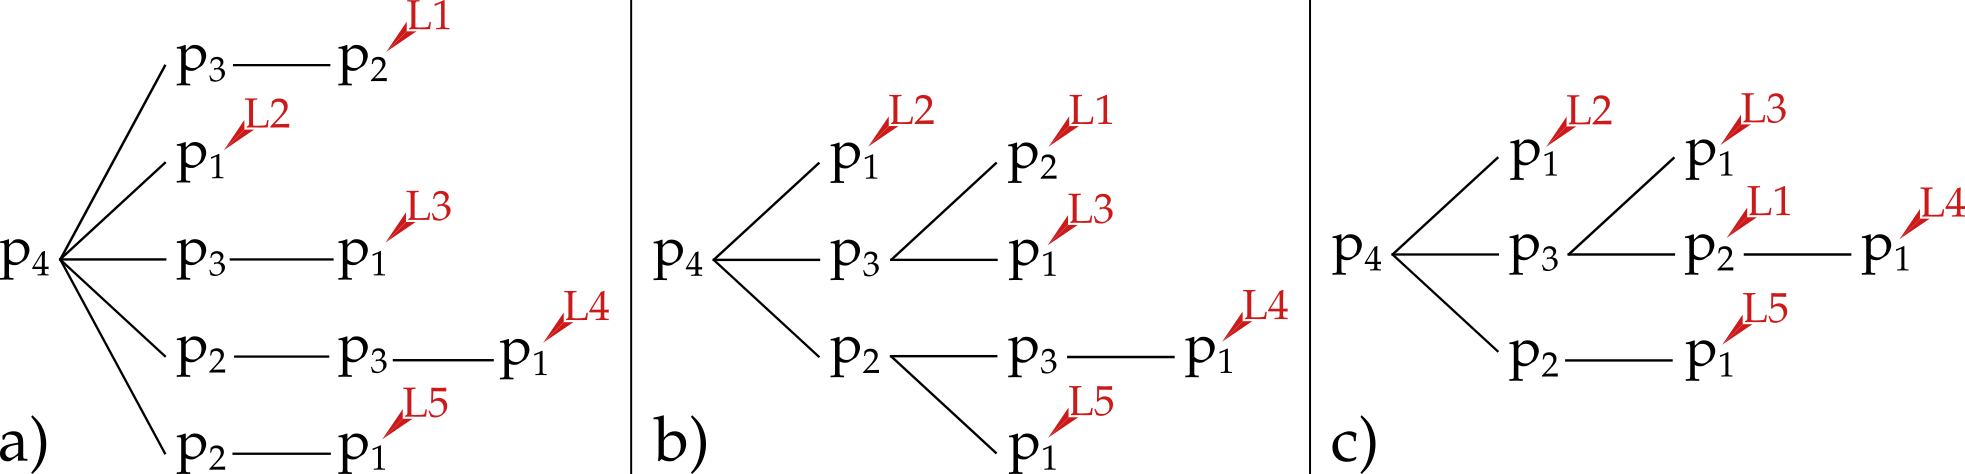
\includegraphics[width=\textwidth]{figures/chapter7/naive.png}
\caption{\label{fig:chap7_naive} Two naive trie representations of the family of subsets extracted from properties involved in the label patterns. The trie a) considers the subject property as the root of the tree and creates a branch for each label pattern respecting the order of apparition of the properties. The trie b) takes the same construction rule as the a) but merges the common children of each node. The trie c) is the same principle of b) but the elements $p_2$ and $p_3$ have been switched for L4. While the two first tries have a width of five, the last has a width of four.}
\end{figure}

\subsubsection{Advanced strategy to explore compound relations}

To find a strategy to create a trie minimizing the width, we first have to study the characteristics of the family of sets.
The first axiom that we can do on the subsets of our family is that they are neither totally ordered, as we can explore their element in any order, or partially ordered, as we can not compare their members. Therefore, we cannot use the tools of the order theory such as the Hasse diagram. Taking a look at mathematical approaches of tree-representation of set families~\cite{bui_2008_tree}, we face the problem that our set family does not respect some essential properties. For each pair $(A, B)$ of sets of $S$, we can not ensure that one of the following rules is true : $A \cap B \neq \emptyset$, $A \cap B \neq A$, or $A \cap B \neq B$. This means that we cannot ensure that each pair of sets are either disjoint or related by containment. Wherefore, our family $F$ is not a laminar set family.
Moreover, for each pair $(A, B)$ of sets of $S$, we can not ensure that their intersection is non-empty ($A \cap B \neq \emptyset$), neither that their difference are non-empty ($A \setminus B \neq \emptyset$ and $B \setminus A \neq \emptyset$). Wherefore, our family $F$ is not a cross-free or an overlap-free family but it does not mean that it is an intersecting and crossing family.

To limit our problem, we do a first assumption. Because the subject property $\property_s$ is the one having introduced the \acrshort{cr}, we can assume that this property has already been selected among the others. Moreover, it will always be the common element of all the sets of the family. We thus consider it as the root node of the exploration tree and remove it from every set of the family $S$ giving a new family:

\begin{align*}
S' = \{A\ |\ A = X \setminus \property_s,\ \forall X \subseteq S\}
\end{align*}

From there, we need to find the child nodes of the root in a way to minimize their number and that every subset of $S'$ has at least one of their element attached to one of the child nodes. This sub-problem is a specification of the Hitting Set problem. It is defined as follows. Giving $F = \{S_1,S_2,...,S_m\}$ the collection of subsets of $S$ (i.e. $S_i \subseteq S, \forall i$) and a natural number $k \in \field{N}$, we want to know if exists $S' \subset S$ where $|S'| < k$ such that $S_i \cap S' \neq \emptyset, i = 1,2,...,m$. In our case, we are searching $k$ as to be as small as possible. In some way, the Hitting Set problem can be seen as a Set Covering problem, shown to be NP-complete~\cite{karp_1972_reducibility}. To avoid any combinatorial explosions, we thus propose a greedy algorithm.

Giving a node $n_i$ of the tree and it related family of set $S$, the quantity $|\{S_j \in S ~|~ x_i \in S_j \}|$ is the frequency of the element $x_i$ in $S$. Among the elements of the universe of the current node $n$, we select $x_{max}$, the element with the highest frequency and create a child node with it. The family related to this new node is computed with the equation~\eqref{eq:chap7_child_family} and the family related to the current node is updated with the equation~\eqref{eq:chap7_node_family_update}. These steps are repeated while $S$ is non-empty to create all the children of the current node and all this process is repeated for each created child nodes until it is possible.

\begin{equation}
S' = \{S_j \setminus x_{max}, S_j \cap \{x_{max}\} \neq \emptyset, \forall S_j \in S\}
\label{eq:chap7_child_family}
\end{equation}

\begin{equation}
S \leftarrow \{S_j, S_j \cap \{x_{max}\} = \emptyset, \forall S_j \in S\}
\label{eq:chap7_node_family_update}
\end{equation}

The tree resulting from this process is represented in Figure~\ref{fig:chap7_advanced} for the purchase example. In the root node with the property $p_4$, the element with the highest frequency is $p_1$. We thus create a child node with this property and create its family. Updating the family of the root node, the family only contains the set $\{p_2, p_3\}$. Both having the same frequency, one is chosen over the other, here $p_3$, and we create a new child node. After an update of the family of the root, it will be empty and all the children of the root have been created. The process is repeated for the two created nodes.

\begin{figure}[ht!]
\centering
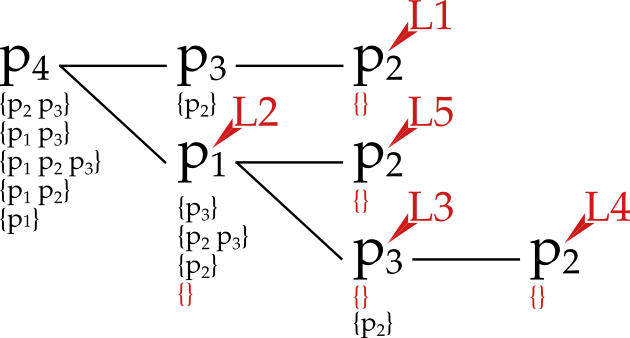
\includegraphics[scale=0.45]{figures/chapter7/advanced.png}
\caption{\label{fig:chap7_advanced} The trie with reduced width, representing all the labels of a compound entity in terms of involved properties. Each node is a property to explore. Attached to each node is the family of subsets that has to be decomposed. An empty set in a family related to a node (in red) signified that one of the initial subsets is fully represented in the trie meaning that all the properties of a pattern will be explored by reaching this node. The width of the trie is three against five for the naive version.}
\end{figure}

In the following, such search-tree will be referred to as a \acrfull{ct}. Taking a part of it (i.e. taking one of its nodes as a local root) gives a sub-\acrshort{ct}.

\section{REG with compound relations}

Thanks to the \acrshort{ce} labels analyse, we have created a search-tree to lead the exploration of \acrshort{cr} in the \acrshort{reg} algorithm. In this section, we present the modification we made to use \acrshort{cr} in the \acrshort{reg} algorithm. The core of the algorithm based on the Uniform Cost Search algorithm is unchanged and is recalled in algorithm~\ref{alg:chap7_ucs}.

\begin{algorithm}[!ht]
\caption{Uniform-Cost Search algorithm for Referring Expression Generation}
\label{alg:chap7_ucs}
\begin{algorithmic}
\Function{UCS\_REG}{$problem$} 
    \State $node\leftarrow$ a node with RE = \textsc{create-initial-re}(\textit{problem}.context), \textit{cost} = 0
    \State $frontier\leftarrow$ a priority queue of nodes ordered by their \textit{cost}
    \State $frontier\leftarrow$ \textsc{INSERT}($node$, $frontier$)
    \State $explored\leftarrow$ an empty set
    \Loop
        \If{\textsc{empty}($frontier$)} 
        	\State \Return failure
        \EndIf
        \State $node\leftarrow$ \textsc{pop}($frontier$)
        \If{\goaltest($problem$, \toquery($node$))} 
        	\State \Return \textsc{SOLUTION}($node$)
        \EndIf
        \State add $node.RE$ to $explored$
        \ForAll{$addition$ in \additions($node$)}
            \State $child \leftarrow \createchild(node, addition)$
            \If{$child.RE$ is not in $explored$ or $frontier$}
            	\State $frontier\leftarrow$ \textsc{INSERT}($child$, $frontier$)
            \EndIf
        \EndFor
    \EndLoop
\EndFunction
\end{algorithmic}
\end{algorithm}

\subsection{Exploring the compound relations}

At the difference of the tasks descriptions of the previous chapter, the current algorithm can not have any prior knowledge about the relations leading to the use of \acrshort{cr}. A \acrshort{cr} can only be discovered if a relation introduces a \acrshort{ce}. However, an entity can be said to be a \acrshort{ce} only thanks to the labels of one of its upper class. With regard to this information, we cannot have any function dedicated to the addition of \acrshort{cr} and each newly introduced entity in a candidate \acrshort{re} has to be tested to assess if it is a \acrshort{ce} or not.

The analyse of the entities' labels and their usable classes, meaning their upper classes having labels, is an already existing process in the \acrshort{reg} algorithm. It is performed by the function $\typingadditions$ of algorithm~\ref{alg:typing_action}. It initially aims at satisfying the parlance need constraint. With some modifications, the $\typingadditions$ will be used to detect any newly introduced \acrshort{ce} by testing if the labels of the usable classes are in the form of a pattern. If they are it returns the detected \acrshort{ce}. To do so, the \textit{additions} are now composed of a relation to be added and a \acrshort{ce} in one has been found.

Once \acrshort{ce}s have been detected, we have to create a \acrfull{ct} for each in order to lead the \acrshort{reg} search process. To each node of the \acrshort{reg} algorithm, in addition to the candidate \acrshort{re} and its associated cost, we introduce a map of \acrshort{ct}s. This map link a \acrshort{ce} involves in the candidate \acrshort{re} related to the node to its \acrshort{ct} or one of its sub-\acrshort{ct}. The management of these trees is done by the $\createchild$ that has been modified (see algorithm~\ref{alg:chap7_child}. If the addition introduces a new \acrshort{ce}, we create it related \acrshort{ct}\footnote{For performance gain, all created \acrshort{ct} can be stored in a collection of \acrshort{ct} in order to compute them only once even if the same \acrshort{ce} is introduced in two disting branches of the \acrshort{ucs}.}. Otherwise, with the function $\getsubtrees$ we test is the new relation corresponds to one of the branches of one of the \acrshort{ct}s of the parent node. If it is, we take the sub-\acrshort{ct} corresponding to the relation. Taking the entity $\indiv_c$ as introduced \acrshort{ce} through the relation $(\indiv_4, \overline{\property_4}, \indiv_c)$, the \acrshort{ct} of figure~\ref{fig:chap7_advanced} is first created. If in a second time the relation $(\indiv_c, \property_1, \indiv_1)$ is inserted, $\createchild$ would take the sub-\acrshort{ct} having $\property_1$ as root.

\begin{algorithm}[ht!]
\caption{\label{alg:chap7_child} Child node function modified to use compound relations.}
\begin{algorithmic}
\Function{\createchild}{$addition$, $parent$} 
    \State \Return a node with
    \State RE = $parent$.RE $\cup$ $addition$.relation
    \State cost = $parent$.cost + $\costfunc(addition$.relation$)$
    \If{$addition$.CE}
    	\State CTs $\leftarrow$ INSERT($\createtree(addition$.CE$)$, $parent$.CTs)
    \Else
    	\State CTs $\leftarrow$ $\getsubtrees$($addition$.relation, $parent$.CTs)
    \EndIf
\EndFunction
\end{algorithmic}
\end{algorithm}

At this stage, we detect the introduction of \acrshort{cr} and manage the \acrshort{ct}s. The $\additions$ can now use the \acrshort{ct}s to propose new additions. As describe with the algorithm~\ref{alg:chap7_additions}, we keep the two functions $typingadditions$ and $\differenceadditions$. We introduce a new function $\compoundadditions$ aiming to complete the \acrshort{cr} having been started. For each \acrshort{ct} of the node it propose the relation of the form $(\indiv_c, \property_i, \indiv_i) \in \relationset$ such that the properties $\property_i$ are the branches of the root of the \acrshort{ct} related to $\indiv_c$. With the  \acrshort{ct} of figure~\ref{fig:chap7_advanced}, the $\compoundadditions$ function would generate two addtions being $(\indiv_c, \property_3, \indiv_3)$ and $(\indiv_c, \property_1, \indiv_1)$.

\begin{algorithm}[ht!]
\caption{\label{alg:chap7_additions} The modified $\additions$ function modified to use compound relations. }

\begin{algorithmic}

    \Function{\additions}{$node$} 
        \State $sucess, additions\leftarrow$ \typingadditions($node$)
        \If{$sucess = True\ and\ additions \neq \emptyset$}
            \Return $additions$
        \EndIf
        
        \State $additions\leftarrow$ \compoundadditions($node$) \Comment{new introduced function}
        \State $additions\leftarrow additions\ \cup$ \differenceadditions($node$) 
        
        \Return $additions$
    \EndFunction
    
\end{algorithmic}
\end{algorithm}

\subsection{Determining a referring expression validity}

Going back to the original definition of the \acrshort{reg} problem, a \acrshort{re} is valid if the parlance need is satisfied (theorem~\ref{the:parlance_need}), all the introduced variables can be intantiated (theorem~\ref{the:correct_intance}), and the variable representing the target entity can only be bound to the target entity (theorem~\ref{the:re_mini_validity}) for a minimal validity.

For the compound relations, their validity criteria is that we can use onr of their labels to speak about them. In other words, taking all the relations involving a given \acrshort{ce}, we must be able to rebuild one of his family's sets. Each of its \acrshort{cr} thus has to be complet (see theorem~\ref{the:cd_completion}).

\begin{theorem} [The CR completion]
\label{the:cd_completion}
A \acrshort{cr} of family $S$ is said to be complet iif given its \acrshort{ce} $\indiv_c$ we can create, from the set of relation $\mathcal{T}$ representing a candidate \acrshort{re}, a set $v = \{\property_i\ |\ (\indiv_c, \property_i, \indiv_i) \in \mathcal{T} \lor (\indiv_i, \overline{\property_i}, \indiv_c) \in \mathcal{T} \}$ such that $v \subset S$.
\end{theorem}

From a technical point of view, such constraint can be hard to compute for each node to be tested. However, during the creation of a \acrshort{ct}, this information can already already known. During the \acrshort{ct} creation, each time a child node is created with an empty set its family of sets, this means that a label of the \acrshort{cr} is represented in its entirety at this node. On the figure~\ref{fig:chap7_advanced} the completed labels are represented by the red arrows. We can thus store this information in the \acrshort{ct} nodes. Because during the \acrshort{reg} search process we cut down these trees taking each time a sub-\acrshort{ct}, we just have to test if each current root of the \acrshort{ct}s of the node to test can represent a label or not. If all can, the candidate \acrshort{re} of the current node is valid regaring the \acrshort{cr} completion.

\subsection{From tree to radix tree}

A limitation identified from the previous chapter was the addition of a single relation at each step while we can know that the candidate \acrshort{re} will not be valid because of the completion constraint. With the present method using multiple labels not involving all the relations, the limitation has been partially solved. In addition, thanks to the \acrshort{ct}, the branching factor is limited and even if an addition does not lead to a valid \acrshort{re}, it will be used for several labels. However, in some cases, this limitation still appears. Considering the \acrlong{ct} of figure~\ref{fig:chap7_advanced}. Starting from the root node $\property_4$, we can go to the nodes $\property_3$ and $\property_1$. While the node $\property_1$ create a complete \acrshort{cr} and make a step toward another complete \acrshort{cr}, the node $\property_3$ does not. It makes a step toward the single label $L1$ but does not complete it.

To solve this issue, we can use the radix tree structure, also called compact prefix tree. It consists of merging each node that is the only child with its parent if the parent node does not represent a valid label. In the example of figure~\ref{fig:chap7_advanced}, the node with the property $\property_2$ could thus be merged with its parent $\property_3$.

The major consequence of such modification is that the additions have to no more represent a single relation but a set of relations. Even if it makes the additions comparison harder to compute it reduce the overall branching factor. Keeping our example, if we add at once the relation involving $\property_2$ and $\property_3$ and that both introduce an anonymous entity, this means that at the next step the $\typingadditions$ function could type both at once. Where previously these additions would require four steps, and thus branching at each, with this solution it only required two.

\section{Results}

In this section, we present some result of the \acrshort{reg} with compound relations. We start with the introduction example of Sean Connery's performance. Then we give performance measures using the setup of the previous chapter in order to assess the impact of the proposed modifications. 

\subsection{The actor playing James Bond}

For this simple test, we describe actor performance using the pattern of figure~\ref{fig:chap7_perf}. Both the actor and the film can be used as a subject of the \acrshort{cr} thanks to the presence of inverse properties. The set of labels attached to the \textit{Performance} class is listed in listing~\ref{lst:chap7_perf_labels}. Three are available to describe the actor and two (equivalent) for the film.

\begin{figure}[ht!]
\centering
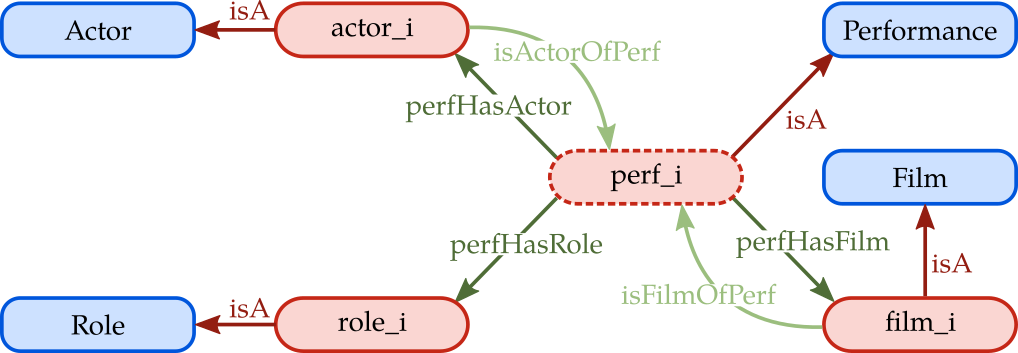
\includegraphics[scale=0.4]{figures/chapter7/perf.png}
\caption{\label{fig:chap7_perf} The compound relation patten used to discribe a performance of an actor with a role and a film.}
\end{figure}

\begin{lstlisting}[frame=single, caption={ The set of labels usable to discribe the performance compound relation.}, label={lst:chap7_perf_labels}, captionpos=b, style=Labels, mathescape=true]
L1 - {?perfHasActor} who played {perfHasRole} in {perfHasFilm}
L2 - {?perfHasActor} who played {perfHasRole}
L3 - {?perfHasActor} who played in {perfHasFilm}
L4 - {?perfHasFilm} in which {perfHasActor} play {perfHasRole}
L5 - {?perfHasFilm} in which {perfHasRole} is played by {perfHasActor}
\end{lstlisting}

We first create an ontology describing two performances. The performance \textit{perf\_sean} link the actor \textit{sean\_connery} with the role of \textit{james\_bond} and the film \textit{gold\_finger}. The second is \textit{perf\_craig} with \textit{daniel\_craig} in the role of \textit{james\_bond} and in the film \textit{casino\_royale}. The individuals representing the films and the roles have labels while the others do not. Running our algorithm on this ontology we get the result:

\begin{gather*}
(?0,\ isA,\ Actor),\\
(?0,\ isActorOfPerf,\ ?1),\\
(?1,\ isA,\ Performance),\\
(?1,\ perfHasFilm,\ gold\_finger)
\end{gather*}

Matching it the the ontology, the variable \textit{?0} matchs \textit{sean\_connery} and the variable \textit{?1} matchs the performance \textit{perf\_sean}. Adding the performance \textit{perf\_gert} linking the actor \textit{gert\_frobe} with the role of \textit{auric\_finger} and the film \textit{gold\_finger} the previous solution is no more valid. Running the algorithm on the new ontology, we get the result:

\begin{gather*}
(?0,\ isA,\ Actor),\\
(?0,\ isActorOfPerf,\ ?1),\\
(?1,\ isA,\ Performance),\\
(?1,\ perfHasFilm,\ gold\_finger),\\
(?1,\ perfHasRole,\ james\_bond)
\end{gather*}

With this simple example we see that with a single compound relation, the algorithm is able to find a solution by selecting the necessary information in it depending on the situation while keeping the link between each of them.

\subsection{The desciption of past activities as compound relations}

Since the presented algorithm is able to manage the past tasks description, we present a comparison in terms of execution time with both the original algorithm and the one using past tasks. To do so, take the knowledge base of the previous chapter containing two task description per entity inheriting from the \textit{Object} class. To be used with compound relations, we add a label to each class representing a task. The label involves the three parameters of the task. In this way, we reproduce the constraint to use all the parameters and at the same time take advantage of the radix-tree optimisations. The knowledge base is still managed using the Ontologenius system and not passing by the ROS services to not be impacted by the communication time in our measures.

\begin{figure}[ht!]
\centering
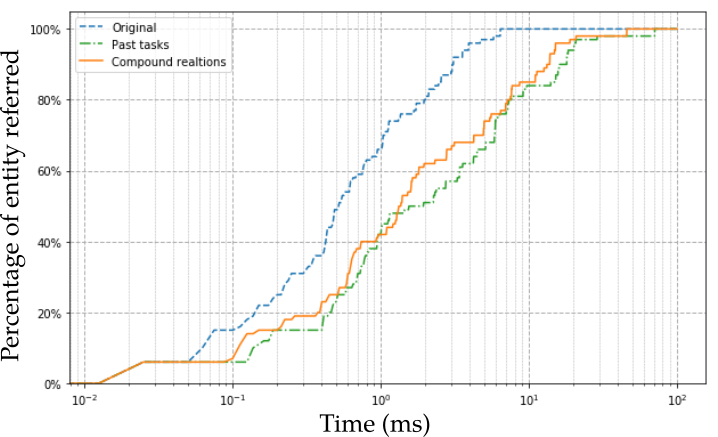
\includegraphics[scale=0.5]{figures/chapter7/comparison.png}
\caption{\label{fig:chap7_compare} Comparison of the three algorithms regarding the percentage of successfully referenced entities over time using a logarithmic timescale. }
\end{figure}

The original algorithm has been run without the possibility to use relations toward task since it is not designed for this use. Its performance is our comparison point as we expect all algorithms to find the same solutions. For recall, the described tasks are designed in such a way to not help in the \acrshort{re} generation and but ourselves in the worst case. The measures of the percentage of entities referred over time for all three algorithms are represented in Figure~\ref{fig:chap7_compare} and reported on appendix~\ref{app:reg_comp_solutions}.

With this setup, the current version performs slightly better than the previous one with an average resolution time of 4.17ms versus 5.53. It is however over the original version having an average resolution time of 1.08ms. This difference must be qualified by the exploration of \acrshort{cr}s that the original one does not do. While the majority of the entities are referred in a comparable time with the previous version, we can still note that the more complex entity requiring six relations is now solved in 45.71ms versus 70.57ms previously.

An advantage of the current algorithm is that in the case no \acrshort{cr}s are described the performance are the same as the original algorithm. At the difference, the previous version had an impact even if negligible. 

% chap 4
%count    77.000000
%mean      1.080750
%std       1.355236
%min       0.013237
%25%       0.193782
%50%       0.516371
%75%       1.322064
%max       6.405807

% chap 6
%count    77.000000
%mean      5.531283
%std       9.780631
%min       0.012952
%25%       0.509738
%50%       1.538461
%75%       5.968753
%max      70.577606

% chap 7
%count    77.000000
%mean      4.178141
%std       6.855033
%min       0.016902
%25%       0.438766
%50%       1.323878
%75%       5.447168
%max      45.716713